% Chapter Template

\chapter{Optimisation de tâches} % Main chapter title

\label{Chapitre 4} % Change X to a consecutive number; for referencing this chapter elsewhere, use \ref{ChapterX}

\lhead{ \emph{Optimisation de tâches}} % Change X to a consecutive number; this is for the header on each page - perhaps a shortened title

Ce dernier chapitre nous explique par l'exemple qu'une application peut être drastiquement améliorée si l'on analyse correctement son fonctionnement dynamique. Vous le verrez par vous mêmes. 

%----------------------------------------------------------------------------------------
%	SECTION 1
%----------------------------------------------------------------------------------------
\section{Exemple d'application}
Pour cette partie, l'idée est de capturer des image sur une caméra et de l'afficher sur le petit écran de notre cible  AFP-27. Pour cela nous utilisons une caméra C310 de Logitech (qui par ailleurs est capable de fournir 720p à 30 fps). Comme vous pourrez le constater le programme fourni n'est vraiment pas très performant. Mettons nous d'accord sur une résolution d'image de 320x240 pixels, car les performances dépendent directement de celle-ci.\\

Le programme de base nous est fourni, et le but est évidement de l'optimiser le plus possible.

\pagebreak \section{Analyse du programme}

\subsection{Consommation CPU}
Pour commencer, lançons simplement le programme et regardons sa consommation CPU. A l'aide de notre fidèle fonction "top", voici ce qu'on obtient :
\begin{center} 
\hspace{12.45cm}
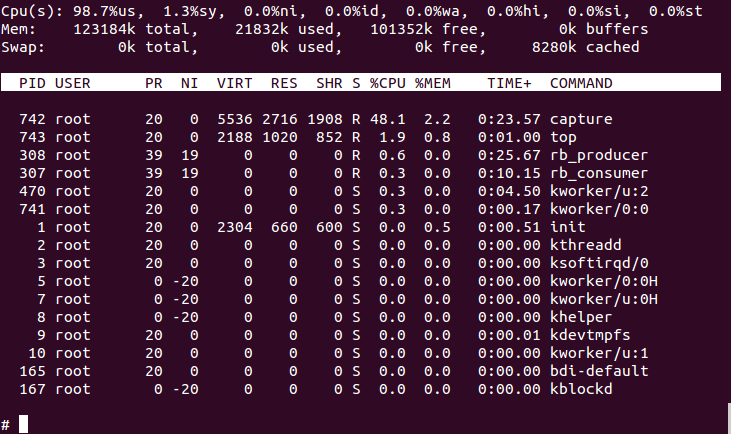
\includegraphics[width=17cm]{top_non_opt.png}
\end{center}
\vspace{0.5cm}

On voit que le processus prend 48.1\% de la CPU (qui est utilisée à 98.7\% au total). Pour information, un démon (compteur) lancé au démarrage "bouffe" le reste de notre CPU. Nous avons ajouté à ceci une mesure de la vitesse. A ce point nous n'avions pas encore mis sur pied la mesure des "fps". A ce point, il faut essayer de regarder qu'est-ce qui prend du temps dans notre application.



\pagebreak \subsection{Strace}

Pour voir un peu ce que fait notre programme, nous l'avons tracé avec l'outil "strace". Voilà le résultat de cette analyse :

\begin{center} 
\hspace{12.45cm}
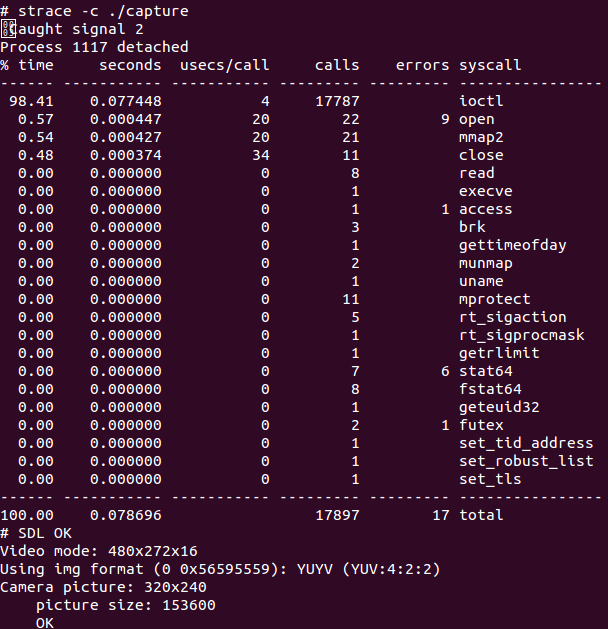
\includegraphics[width=17cm]{strace_capture.png}
\end{center}
\vspace{0.5cm}

On voit beaucoup d'accès "ioctl", ce qui est normal vu que l'on accède à un module noyau qui pilote la caméra. On voit aussi que notre programme travaille avec mmap (pour les "buffers" de données). Ce programme pourrait fonctionner avec les fonctions "read()" et "write()" entre autre. On peut en conclure que le programme lui-même attend "beaucoup" sur des I/Os et donc ne devrait pas trop consommer de ressources CPU. Mais c'est le cas ! Donc voyons plus en détail ce que fait l'application.


\pagebreak \subsection{O-Profile}

Un outil est disponible dans le "framework" buildroot pour nous aider à édifier le profil d'un programme. Cet outil se nomme "o-profile", et il faut l'activer dans la configuration de compilation de buildroot (il existe un autre outil "gprof", mais n'est pas disponible sur notre cible). Voilà l'analyse effectuée avec "o-profile" du programme non-optimisé :

\begin{center} 
\hspace{12.45cm}
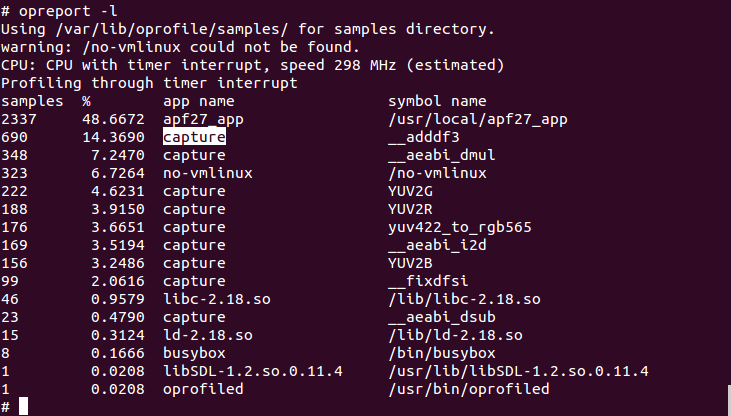
\includegraphics[width=17cm]{oprofile_report.png}
\end{center}
\vspace{0.5cm}

On remarque aisément les routines "adddf3", "aeabi\_dmul", "YUV2G", "YUV2R" et "yuv422\_ to\_ rgb565". Ce qui implique que notre programme effectue des calcul en virgule flottante dans les fonctions nommées précédemment. Voici la routine YUV2R :

\begin{lstlisting}[frame=single,style=C]  % Start your code-block

#define STRIP(X) (X = X > 255 ? 255 : (X < 0) ? 0 : X)

static Uint8 inline YUV2R(int Y, int U, int V)
{
	int R;
	
	R = Y + 1.4026 * (V-128);
	STRIP(R);

	return R;
}
\end{lstlisting}

Donc on voit bien que c'est la que sont effectués les calculs en virgule flottante. Donc il faut maintenant améliorer notre application.

 

\pagebreak \section{Amélioration}

Le but serait de changer les multiplications virgules flottante en entier (ou encore mieux en décalages, mais nous n'avons pas eu le temps de le tester, car les arrondis auraient pu dégrader l'image). Voici notre première idée d'amélioration d'une fonction

\begin{lstlisting}[frame=single,style=C]  % Start your code-block

#define STRIP(X) (X = X > 255 ? 255 : (X < 0) ? 0 : X)

static Uint8 inline YUV2R(int Y, int U, int V)
{
	int R;
	
	R = Y + ((5745 * (V-128)) >> 12);
	STRIP(R);

	return R;
}
\end{lstlisting}

De plus nous avons mis sur pied un système de mesure de "fps". Avec cette amélioration, on peut voir les performances et la consommation diminuer. Voilà cette fois la consommation CPU effective (sans le démon "counter") :

\begin{center} 
\hspace{12.45cm}
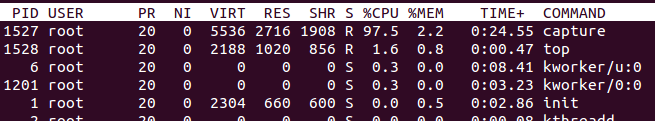
\includegraphics[width=17cm]{top_capture_opt_MMAP.png}
\end{center}
\vspace{0.5cm}

Cette mesure ne nous montre pas de choses extraordinaire, mais cela à considérablement augmenté la fluidité des images (et cela est aussi dû à la mort du démon parasite).

\pagebreak Et voici la mesure avec o-profile avec \textbf{une seule fonction} optimisée. Elle nous permet d'avoir un meilleur aperçu des performance gagnée :

\begin{center} 
\hspace{12.45cm}
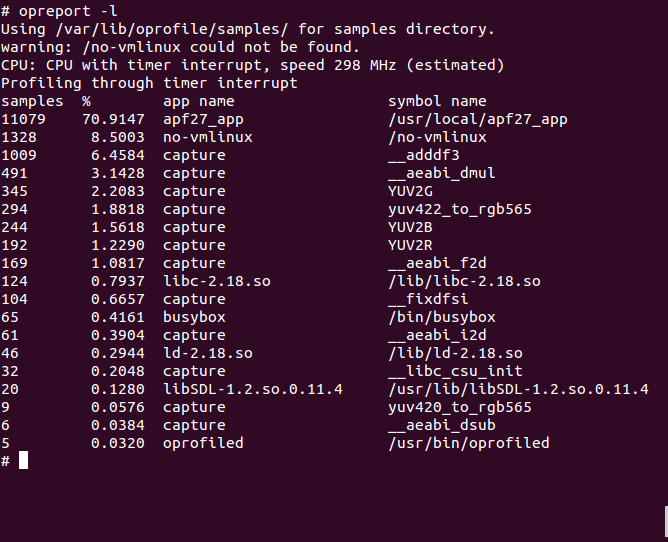
\includegraphics[width=17cm]{opreport_one_optfunc.png}
\end{center}
\vspace{0.5cm}

Au départ "adddf3" prenait 14.36\% du CPU, et cette fois en améliorant, on obtient 6.46\%. Donc juste avec une fonction, nous avons divisé par un facteur plus grand que 2 le temps de calcul en float. Il reste plus qu'à améliorer les autres fonctions.

Voici la vitesse des images (pas très rapide n'est-ce pas ?):

\begin{center} 
\hspace{12.45cm}
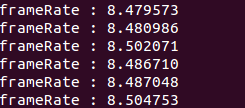
\includegraphics[width=8cm]{lowframerate.png}
\end{center}
\vspace{0.5cm}



\pagebreak Nous avons encore fait une amélioration supplémentaire, c'est de supprimer tout les appels aux fonctions secondaire (YUV2R,...). Voilà le code obtenu :

\begin{lstlisting}[frame=single,style=C]  % Start your code-block

static void yuv422_to_rgb565(void *yuv, int size, void *rgb)
{
	unsigned int yuv32, rgb32;
	int Y, Y2, U, V ;
	int Temp1,Temp2,Temp3;
	int vt128,ut128;
	
	int R, G, B;
	int i;
	Uint32 *dest = (Uint32*) rgb;
	Uint32 *src = (Uint32*) yuv;

	//printf("yuv422_to_rgb565 size : %d\n",size);	

	for (i=size>>2; i; i--)
	{
		yuv32 = *(src++);

		/* packed format */
		Y = (yuv32 & 0x000000ff);
		U = (yuv32 & 0x0000ff00) >> 8;
		Y2 = (yuv32 & 0x00ff0000) >> 16;
		V = (yuv32 & 0xff000000) >> 24;


		vt128 = (V-128);
		ut128 = (U-128);	

		Temp1 = ((179 * (vt128)) >> 7);
		Temp2 = (((11 * (ut128)) - (22 * (vt128))) >> 5);
		Temp3 = ((226 * (ut128)) >> 7);

		R = Y + Temp1;
		G = Y - Temp2;
		B = Y + Temp3;

		STRIP(B);
		STRIP(G);
		STRIP(R);
	
		rgb32 = ((R>>3) << 11) | ((G>>2) << 5) | (B>>3);
		
		R = Y2 + Temp1;
		G = Y2 - Temp2;
		B = Y2 + Temp3;

		STRIP(B);
		STRIP(G);
		STRIP(R);

		rgb32 |= (((R>>3) << 11) | ((G>>2) << 5) | (B>>3)) << 16;

		*(dest++) = rgb32;
	}
}
\end{lstlisting}

Le code pourrait encore être amélioré avec des variables mémorisées dans les registres ("register"). Cette fois-ci, nous avons encore amélioré les performances de l'application.\\

Encore un petit quelque chose, la caméra fournit actuellement un vitesse d'environ 15 images/seconde, et pourtant notre programme n'utilise plus 100\% de la CPU. Donc que ce passe-t-il ? Il faut changer avec des commande "ioctl" du "framework" uvcvideo  (seulement pour certaine résolution dont 320x240)  la vitesse des images. Nous avons donc fait une sorte de "reverse-engineering" sur le programme guvcview, pour connaître les commandes "ioctl" à effectuer. De plus, il faut déscativer l'exposition automatique pour garantir la vitesse (qui s'adapte automatiquement évidemment)

\pagebreak Voilà le code nécessaire :
 
\begin{lstlisting}[frame=single,style=C]  % Start your code-block

static void capture_toggle_auto_exposition(int aVal)
{
	struct v4l2_ext_controls ctrls = {0};
        struct v4l2_ext_control ctrl = {0};
	int ret = 0;
	
	fprintf(stdout,"[capture_toggle_auto_exposition] toggle auto exposition\n");

	// Exposition control
        ctrl.id = 10094851;

	ctrl.value = aVal;

	ctrls.ctrl_class = V4L2_CTRL_CLASS_USER;
        ctrls.count = 1;
        ctrls.controls = &ctrl;
        ret = xioctl(fd, VIDIOC_S_EXT_CTRLS, &ctrls);
        if(ret)
            printf("control id: 0x%08x failed to set (error %i)\n",ctrl.id, ret);
}

void capture_change_framerate(int numerator, int  denominator)
{
	int type = V4L2_BUF_TYPE_VIDEO_CAPTURE;
	int ret = 0;
	struct v4l2_streamparm streamparm;  // v4l2 stream parameters struct

	fprintf(stdout,"[capture_change_framerate] Framerate update\n");

	/*get the current stream parameters*/
	streamparm.type = V4L2_BUF_TYPE_VIDEO_CAPTURE;
	ret = xioctl(fd, VIDIOC_G_PARM, &streamparm);
	if (ret < 0)
	{
		fprintf(stderr, "V4L2_CORE: (VIDIOC_G_PARM) error: %s\n", strerror(errno));
		fprintf(stderr, "V4L2_CORE: Unable to set %d/%d fps\n", numerator, denominator);
	}

	if (!(streamparm.parm.capture.capability & V4L2_CAP_TIMEPERFRAME))
	{
		fprintf(stderr, "V4L2_CORE: V4L2_CAP_TIMEPERFRAME not supported\n");
		fprintf(stderr, "V4L2_CORE: Unable to set %d/%d fps\n", numerator, denominator);
	}

	streamparm.parm.capture.timeperframe.numerator = numerator;
	streamparm.parm.capture.timeperframe.denominator = denominator;

	/*request the new frame rate*/
	ret = xioctl(fd, VIDIOC_S_PARM, &streamparm);

	if (ret < 0)
	{
		fprintf(stderr, "V4L2_CORE: (VIDIOC_S_PARM) error: %s\n", strerror(errno));
		fprintf(stderr, "V4L2_CORE: Unable to set %d/%d fps\n", numerator,denominator);
	}
}
\end{lstlisting}
 
\pagebreak 
De plus, nous avons même testé les fonctions optimisées de conversion yuv422\_rgb565 fourni sous Android :

 
\begin{lstlisting}[frame=single,style=C]  % Start your code-block

/**
*
*	Code from Android : https://android.googlesource.com/device/generic/goldfish/+/master/camera/Converters.h
*
*
*/

/* Clips a value to the unsigned 0-255 range, treating negative values as zero.
*/
static __inline__ int
clamp(int x)
{
if (x > 255) return 255;
if (x < 0) return 0;
return x;
}


/* Build RGB565 word from red, green, and blue bytes. */
#define RGB565(r, g, b) (uint16_t)(((((uint16_t)(b) << 6) | g) << 5) | r)

/* "Optimized" macros that take specialy prepared Y, U, and V values:
* C = Y - 16
* D = U - 128
* E = V - 128
*/
#define YUV2RO(C, D, E) clamp((298 * (C) + 409 * (E) + 128) >> 8)
#define YUV2GO(C, D, E) clamp((298 * (C) - 100 * (D) - 208 * (E) + 128) >> 8)
#define YUV2BO(C, D, E) clamp((298 * (C) + 516 * (D) + 128) >> 8)

/* Converts YUV color to RGB565. */
static __inline__ uint16_t
YUVToRGB565(int y, int u, int v)
{
/* Calculate C, D, and E values for the optimized macro. */
y -= 16; u -= 128; v -= 128;
const uint16_t r = (YUV2RO(y,u,v) >> 3) & 0x1f;
const uint16_t g = (YUV2GO(y,u,v) >> 2) & 0x3f;
const uint16_t b = (YUV2BO(y,u,v) >> 3) & 0x1f;
return RGB565(r, g, b);
}
\end{lstlisting}

Les performance étaient à peu près similaire. Aucune amélioration flagrante n'as été  apporté par rapport à notre code amélioré.

\pagebreak Voici ce que l'on obtient avec une fluidité à 30 fps avec notre code optimisé :

\begin{center} 
\hspace{12.45cm}
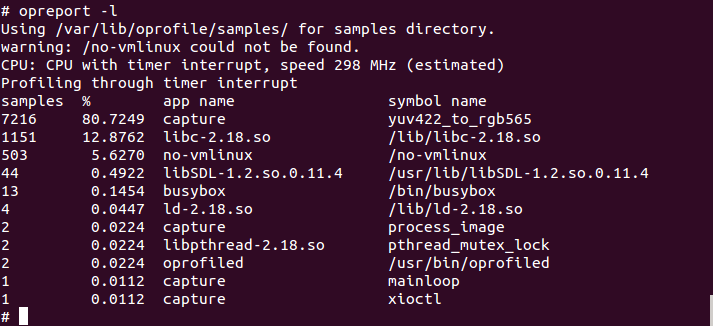
\includegraphics[width=17cm]{opreport_30fps.png}
\end{center}
\vspace{0.5cm}

On voit que pour 30 fps, notre programme consomme un peu plus de 80\% de la CPU. On aimerais descendre au dessous de 40\%. Donc il faut travailler encore.



\pagebreak \section{Assembleur, mon ami !}

Nous avons donc décider d'optimiser la routine en la réécrivant nous même en assembleur. Pour information, nous avons réduit la code d'une centaine de lignes (certes, le code C de cette routine aurait pu être amélioré, mais quand même...). Voici ce code :

\begin{lstlisting}[frame=single,style=C]  % Start your code-block

@ armv6_fast_yuv422_rgb565.s

.section .text
.globl yuv422_to_rgb565
.size	yuv422_to_rgb565, .-yuv422_to_rgb565
.align	2
.type	yuv420_to_rgb565, %function

yuv422_to_rgb565:
	@ args = 0, pretend = 0, frame = 88
	@ frame_needed = 1, uses_anonymous_args = 0
	@ link register save eliminated.
	str	fp, [sp, #-4]!	
	add	fp, sp, #0	
	sub	sp, sp, #92
	asr	r8, r1, #2	@ i = size >> 2
	mov	r1, r0	@ src = yuv
	mov 	r0, r2	@ r0 = dest	
	b	.Lforloop_test		
.Lforloop:
	ldmia 	r1!,{r3} @ => ldr r3,[r1] and add r3,r3,#4
	pld  	[r1,+#4] 	 @ Memory access optimisation
	and	r6, r3, #255	@ Y = (yuv32 & 0x000000ff);
	and	r4, r3, #65280	
	lsr	r4, r4, #8	@ U = (yuv32 & 0x0000ff00) >> 8;
	and	r7, r3, #16711680
	lsr	r7, r7, #16	@ Y2 = (yuv32 & 0x00ff0000) >> 16;				
	lsr	r2, r3, #24	@ V = (yuv32 & 0xff000000) >> 24;	
	sub	r2, r2, #128	@ V = V -128
	sub	r3, r4, #128	@ U = U -128
	mov	r4, #179	
	mul	r4, r2	
	asr	r4, r4, #7	
	str	r4, [fp, #-48]	@ Temp1
	add	r9, r6, r4	@ R = Y + Temp1
	bic	r9, r9, r9, asr #31
	mov	r4,#0xffffff00
	qadd 	r9,r9,r4
	and 	r9,r9,#0xff
	mov 	r4, #11
	mul	r4, r3
	mov 	r5, #22
	mul	r5, r2
	rsb	r4,r5,r4
	asr	r12,r4,#5 	@ Temp2
	rsb	r10, r12, r6	@ G = Y - Temp2
	bic	r10, r10, r10, asr #31
	mov	r4,#0xffffff00
	qadd 	r10,r10,r4
	and 	r10,r10,#0xff
	mov	r4, #226	 
	mul	r4, r3	
	asr	r2, r4, #7	@ Temp3
	add	r4, r2, r6	@ B = Y + Temp3
	bic	r4, r4, r4, asr #31
	mov	r3,#0xffffff00
	qadd 	r4,r4,r3
	and 	r4,r4,#0xff
	asr	r9, r9, #3	@ R >> 3
	mov	r3, r9, asl #11	
	asr	r10, r10, #2	@ G>>2
	add	r3,r3,r10,asl#5 @ r3 = ((R>>3) << 11) | ((G>>2) << 5)
	add	r6,r3,r4,asr#3 @ r6 = (R>>3) << 11) | ((G>>2) << 5) | (B>>3)
	ldr	r3, [fp, #-48]	@ Temp1
	add	r9, r7, r3	@ R = Y2 + Temp1
	bic	r9, r9, r9, asr #31
	mov	r4,#0xffffff00
	qadd 	r9,r9,r4
	and 	r9,r9,#0xff
	rsb	r10, r12, r7	@ G = Y2 - Temp2
	bic	r10, r10, r10, asr #31
	mov	r4,#0xffffff00
	qadd 	r10,r10,r4
	and 	r10,r10,#0xff
	add	r3, r7, r2	@ B = Y2 - Temp3
	bic	r3, r3, r3, asr #31
	mov	r4,#0xffffff00
	qadd 	r3,r3,r4
	and 	r3,r3,#0xff
	asr	r4, r9, #3	@ (R>>3)
	mov	r2, r4, asl #11	@ (R>>3) << 11
	asr	r4, r10, #2	@ (G>>2)
	add	r2, r2, r4, asl #5 @ (((R>>3) << 11) | ((G>>2) << 5) 
	add	r2, r2, r3, asr #3 @ (((R>>3) << 11) | ((G>>2) << 5) | (B>>3))	
	add	r6, r6, r2, asl #16 @rgb |= ()
	stmia	r0!,{r6}
	pld  	[r0,+#4] 	 @ Memory access optimisation
	sub	r8, r8, #1	@ i--
.Lforloop_test:
	cmp	r8, #0	   	@ compare i == 0
	bne	.Lforloop	
	sub	sp, fp, #0	@ else = exit
	@ sp needed	@
	ldr	fp, [sp], #4	@,
	bx	lr	@
\end{lstlisting} 

Voici le profilage avec notre nouvelle optimisation :

\begin{center} 
\hspace{12.45cm}
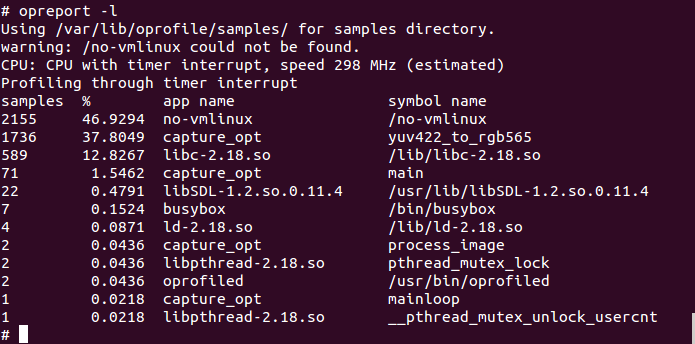
\includegraphics[width=17cm]{opreport_30fps_optasm.png}
\end{center}
\vspace{0.5cm}

Avant, cette routine prenait 80.72\% du CPU, et maintenant elle prend 37.8\% ! On a amélioré la consommation de 40\% pour la même performance ! On pourrait encore imaginer remplacer les multiplications par des opérations à décalage. Mais nous sommes très content et surpris du résultat.  

\pagebreak \section{Optimisation avec le système}

Maintenant on veut que le processus ne consomme pas plus de 40\% de la CPU (comme déjà dit précédemment). Comme on "ne peut plus" améliorer le code, on va essayer de diminuer la vitesse d'images à 25 fps voir 20 fps. Voilà les divers essais (avec 25 fps et 20 fps):
  
\begin{center} 
\hspace{12.45cm}
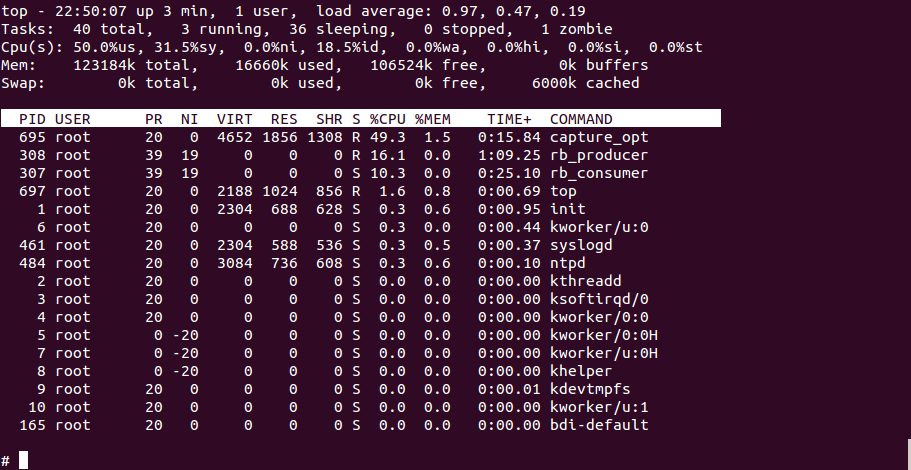
\includegraphics[width=17cm]{top_25fps_opt.png}
\end{center}
\vspace{0.5cm}

  
\begin{center} 
\hspace{12.45cm}
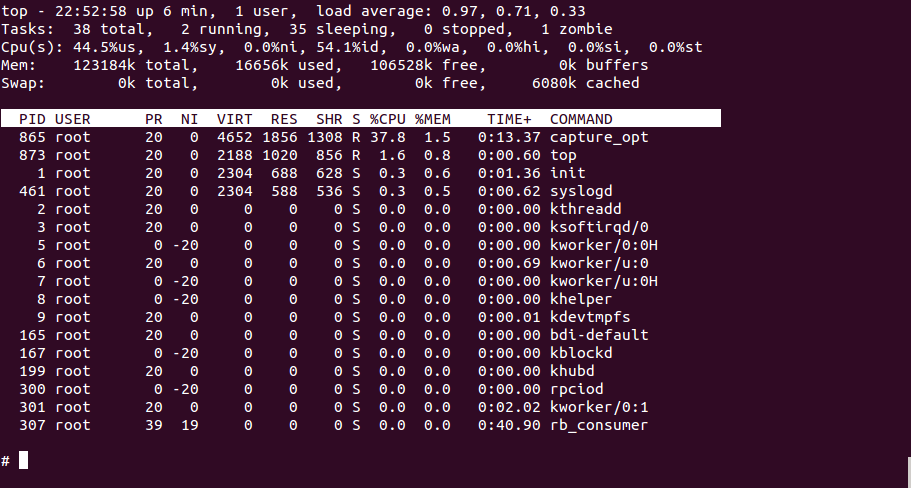
\includegraphics[width=17cm]{top_20fps_opt.png}
\end{center}
\vspace{0.5cm}

On peut voir que on a la bonne consommation à 20 fps. C'est une bonne fluidité pour une consommation relativement faible. Le bon compromis suisse !

\pagebreak Voyons comment se comporte notre programme sur un système chargé. On utilise le processus "yes" plusieurs fois (5x) et voilà le résultat :
 
\begin{center} 
\hspace{12.45cm}
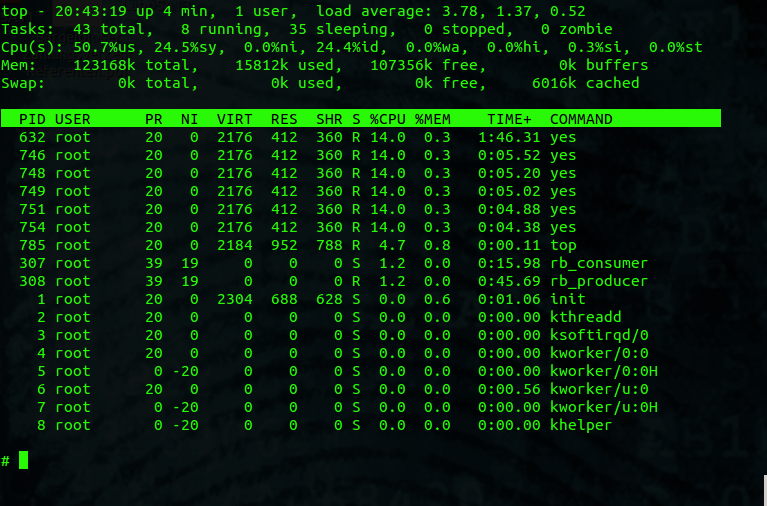
\includegraphics[width=17cm]{yes5_nocgroups.png}
\end{center}
\vspace{0.5cm}

Et si on lance notre application :

\begin{center} 
\hspace{12.45cm}
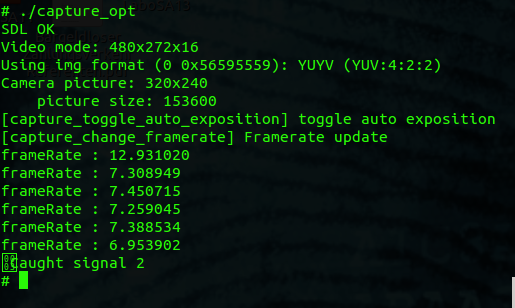
\includegraphics[width=14cm]{capture_opt_load_nocgroups.png}
\end{center}
\vspace{0.5cm}

On voit que le débit est complètement pourri ! Appelons les cgroups à notre secours !

\pagebreak 

Réservons au moins 40\% pour notre programme, et voilà ce qu'on obtient :

\begin{center} 
\hspace{12.45cm}
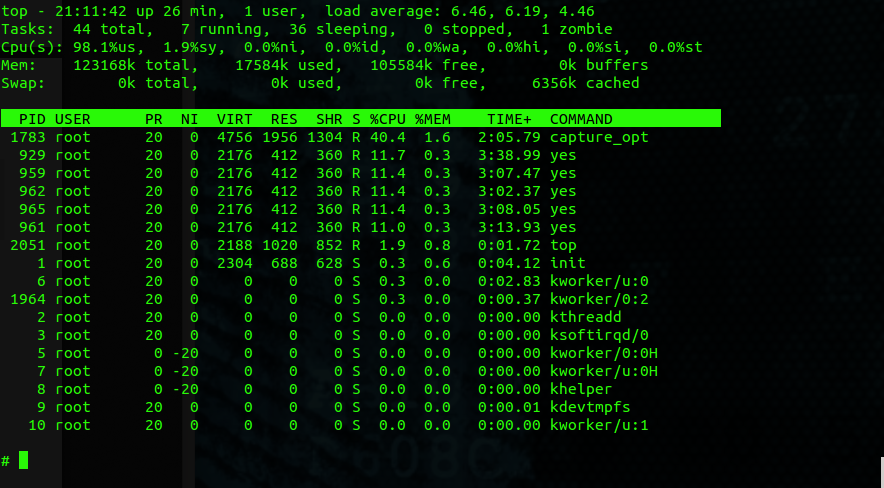
\includegraphics[width=14cm]{capture_cgroup_2048_674.png}
\end{center}
\vspace{0.5cm}

Et si on regarde le nouveau débit, on constate que ça fonctionne magnifiquement bien !

\begin{center} 
\hspace{12.45cm}
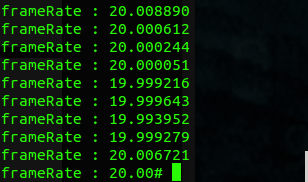
\includegraphics[width=8cm]{capt_framerate_cgroup.png}
\end{center}
\vspace{0.5cm}
